\documentclass[../main.tex]{subfiles}
\begin{document}
\graphicspath{{figures/}{task2/figures/}}

\subsection{Task 2: Player Segment Classification (macro F1)}
\label{sec:t2}

\subsubsection{Problem and Data}

Task 2 asks us to place every player into one of four behavioural segments: \texttt{0} Casual, \texttt{1} Grinder, \texttt{2} Social and \texttt{3} Whale. The metric is \textbf{macro F1}, the unweighted mean of the four per-class F1 scores, so the smallest segment counts as much as the largest. The data used throughout this report is the \textbf{12 November re-release}: the organisers regenerated every Task~2 row, and the \feat{player_id} ordering that had leaked the class in the first release is gone (Section~\ref{sec:t2-mistakes}).

The training set has 104{,}000 rows and the test set 25{,}889 rows. Each row has 44 raw features: 34 numeric columns (play frequency, session length, lifetime playtime, spending, friend counts, ranked and tournament activity, collection progress and similar) and 10 categorical columns, plus \feat{player_id} and the target \feat{segment}. About 7.7\% of the values in each kept feature are missing. We kept 28 of the 44 features (23 continuous and 5 discrete) and dropped the other 16 as pure noise, as Section~\ref{sec:t2-eda} shows.

\subsubsection{EDA Findings}
\label{sec:t2-eda}

We asked four questions. How unbalanced are the classes? Which columns carry any signal? Are the surviving features dependent once the class is known? And how do the four segments relate to each other?

\paragraph{Class balance and missingness.} Figure~\ref{fig:t2-balance} counts the classes and the missing values.

\begin{figure}[H]
\centering
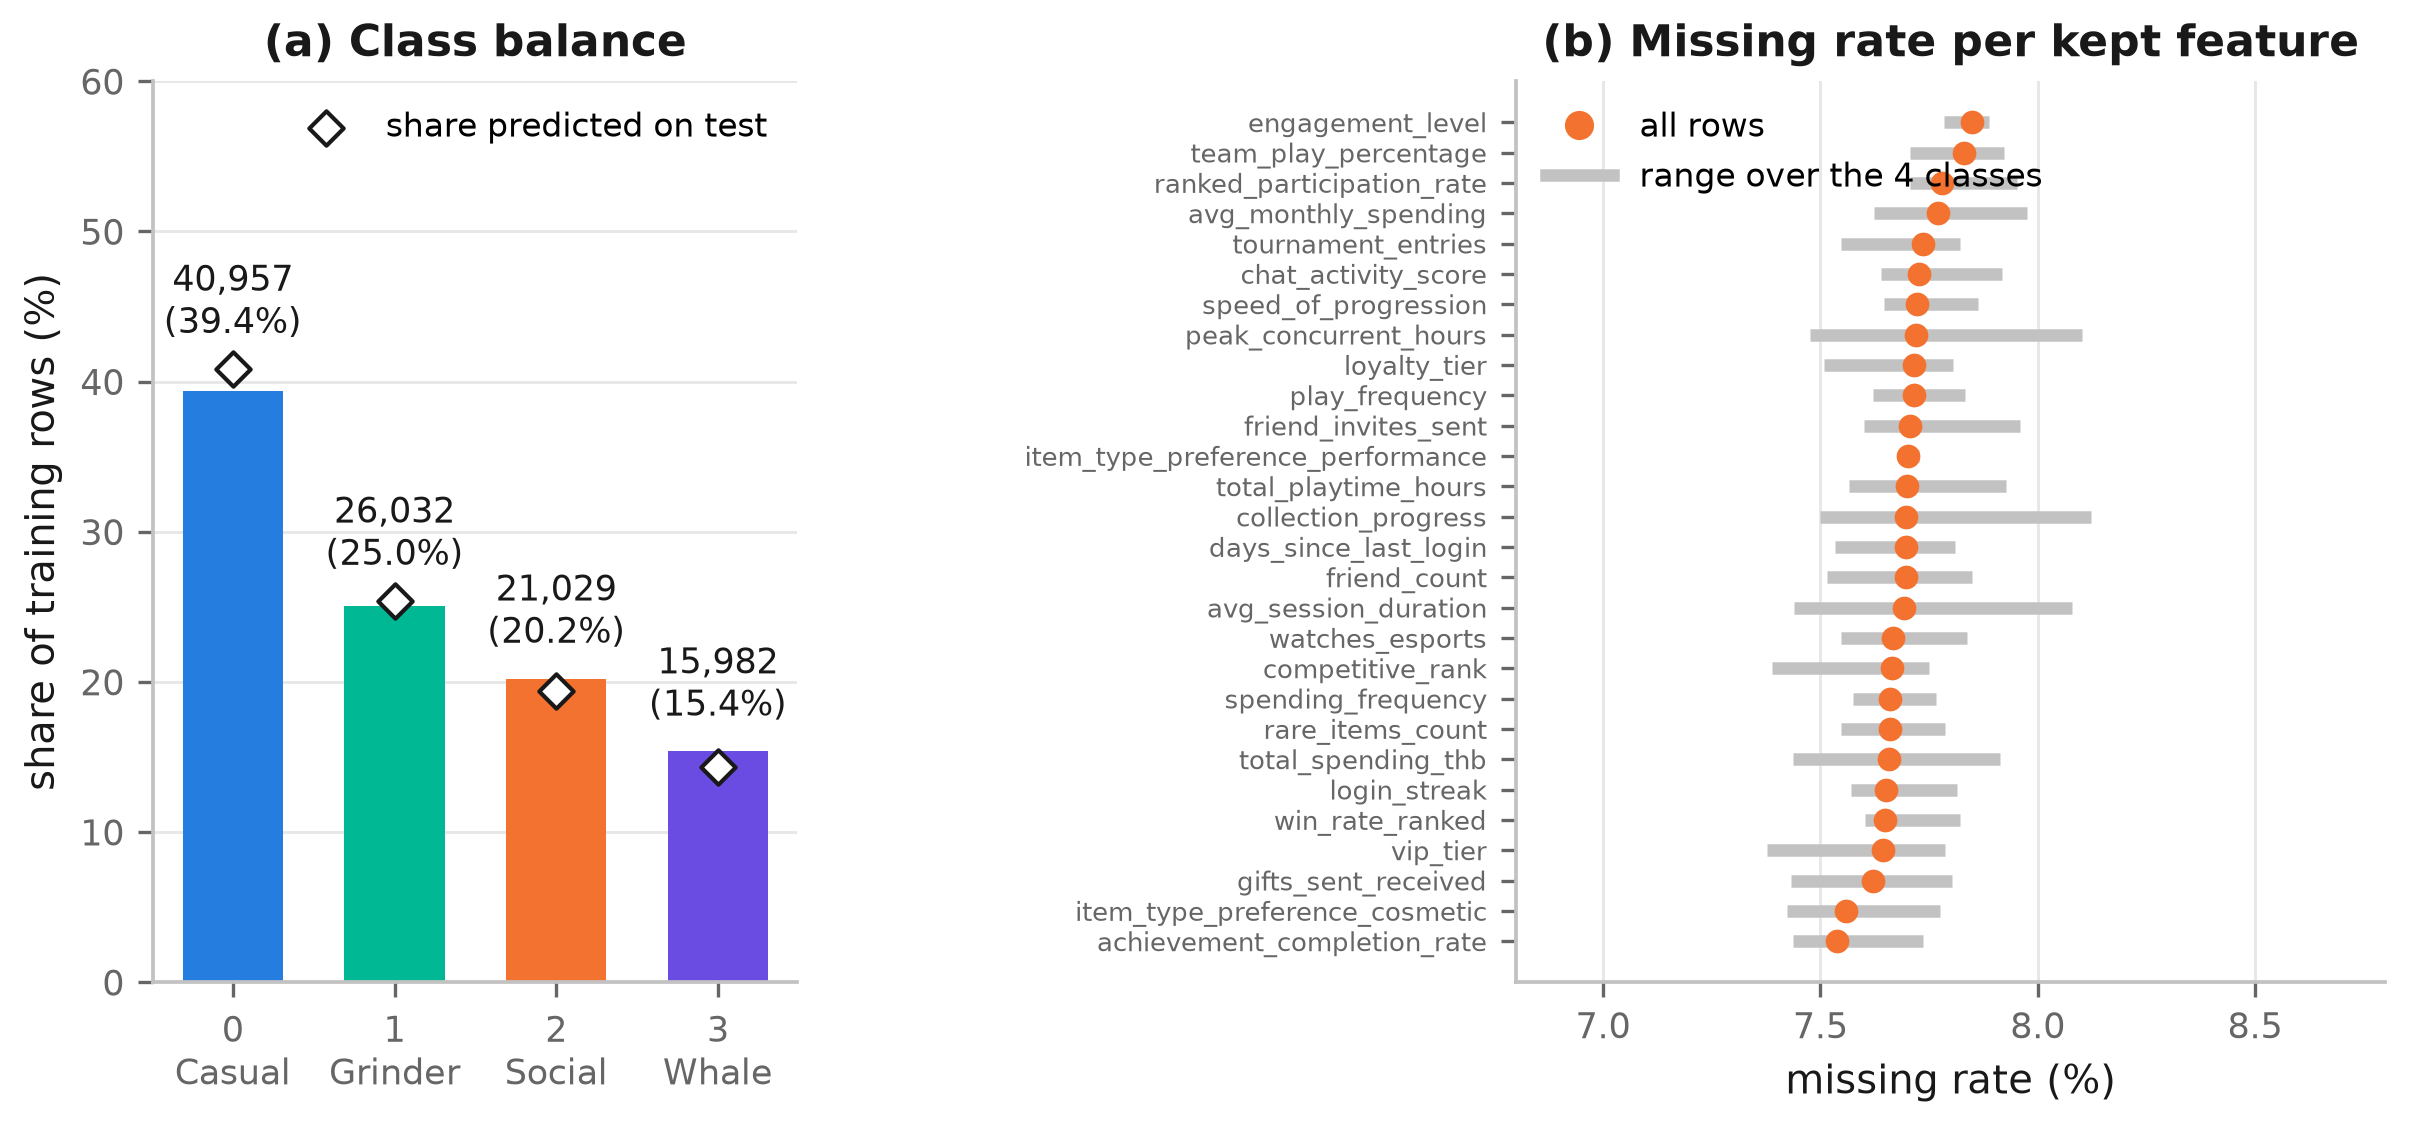
\includegraphics[width=\linewidth,height=0.36\textheight,keepaspectratio]{fig_t2_balance_missing.png}
\caption{(a) Training class balance; diamonds mark the class shares of our final test prediction. (b) Missing rate of each kept feature overall (dot) and across the four classes (grey bar). Segment 0 is 2.6 times as frequent as segment 3, and missingness is about 7.7\% everywhere, independent of the class.}
\label{fig:t2-balance}
\end{figure}

\emph{What we see.} Segment 0 holds 39.4\% of the rows and segment 3 only 15.4\% (Figure~\ref{fig:t2-balance}a). Under macro F1 the rare classes are as valuable as the common one, so a plain \texttt{argmax} will favour class 0. Missingness (Figure~\ref{fig:t2-balance}b) is between 7.54\% and 7.85\% for every kept feature and differs by at most 0.64 percentage points between classes. Nothing in the pattern points to informative missingness. \emph{What we decided.} We fit a decision rule that targets macro F1 directly (Section~\ref{sec:t2-design}) and we treat a missing value as ``no evidence'' rather than imputing it.

\paragraph{Which columns carry signal.} We scored every numeric column with a one-way ANOVA across the four segments and every categorical column with Cram\'er's V (Figure~\ref{fig:t2-signal}).

\begin{figure}[H]
\centering
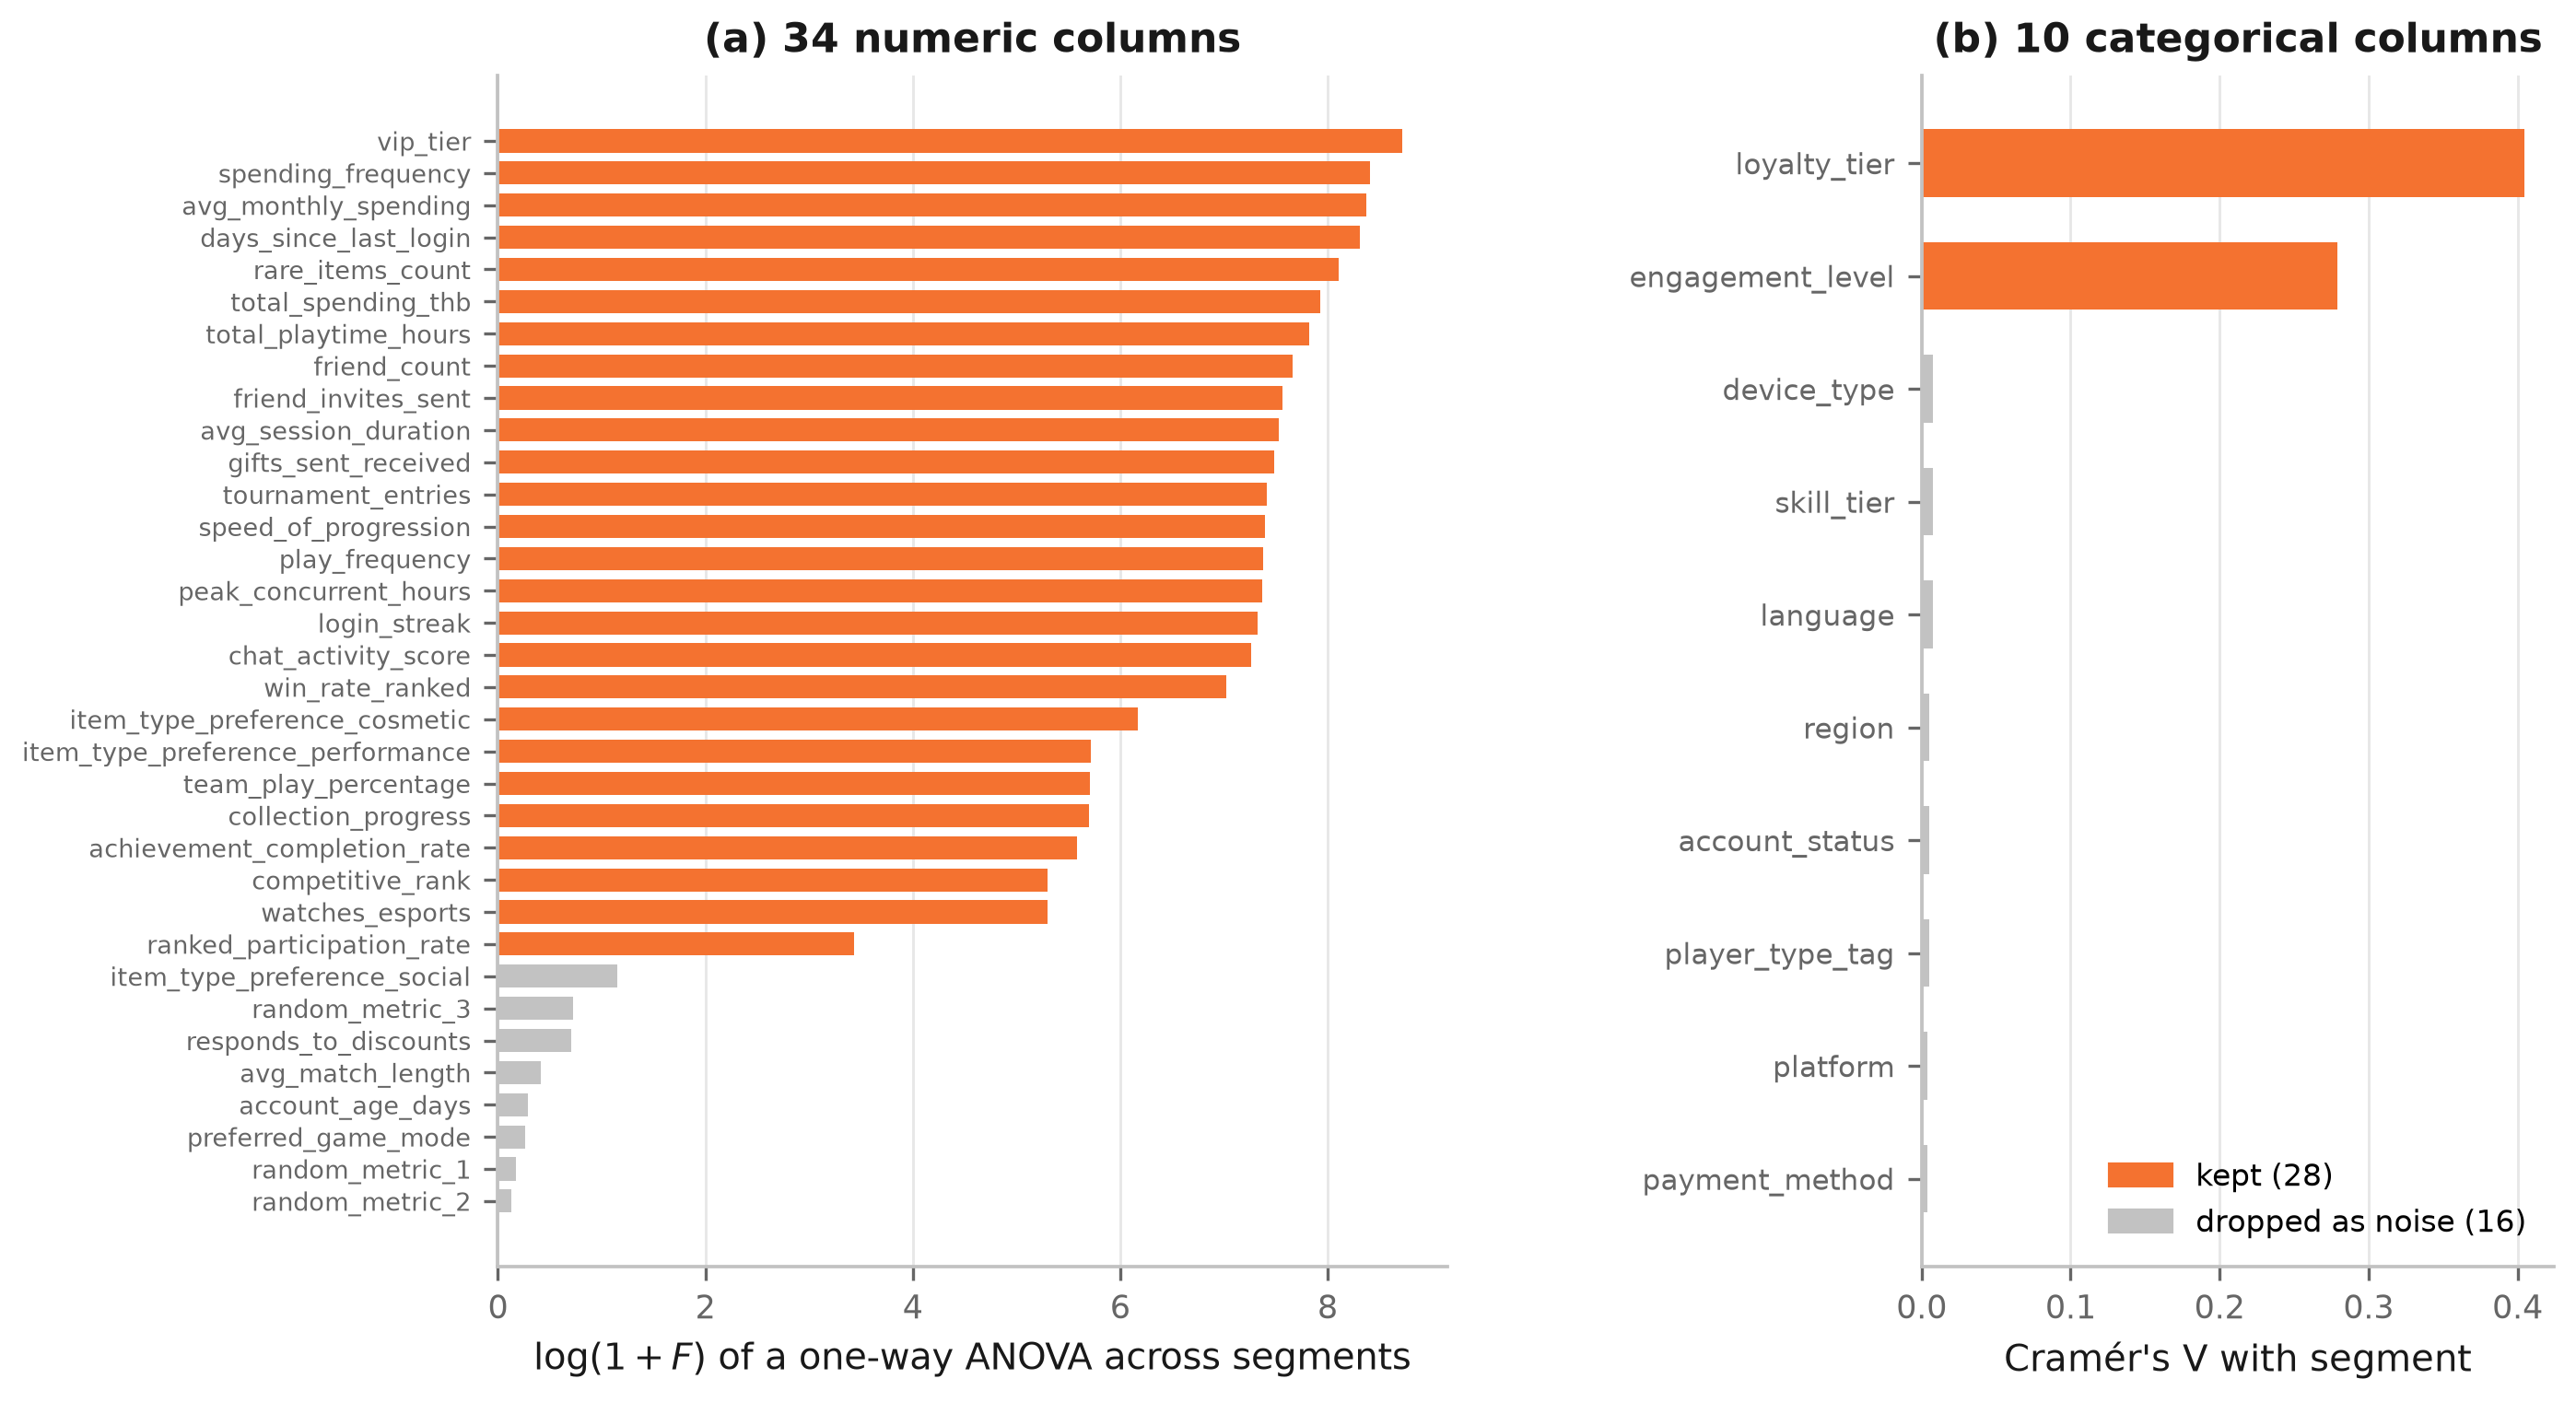
\includegraphics[width=\linewidth,height=0.46\textheight,keepaspectratio]{fig_t2_feature_signal.png}
\caption{Signal of each column against the segment. (a) $\log(1+F)$ of an ANOVA for the 34 numeric columns. (b) Cram\'er's V for the 10 categorical columns. Orange bars are the 28 kept features, grey bars the 16 dropped as noise.}
\label{fig:t2-signal}
\end{figure}

\emph{What we see.} The columns separate into two clean groups. Every dropped numeric column has $\log(1+F)\le 1.15$ and every kept one has $\ge 3.4$. Of the ten categorical columns only \feat{loyalty_tier} (V = 0.404) and \feat{engagement_level} (V = 0.279) matter; the other eight, including \feat{region}, \feat{platform} and \feat{device_type}, have V below 0.008. Three columns are explicitly named \feat{random_metric_1..3}. \emph{What we decided.} Drop \feat{player_id} and the 16 noise columns (8 numeric, 8 categorical). That leaves 28 features, which keeps the models small and stops them from fitting noise.

\paragraph{Independence given the class.} The model choice rests on one question: are the 23 continuous kept features correlated \emph{inside} a class? Figure~\ref{fig:t2-indep} compares the Spearman correlation of all rows with the class-weighted average of the four within-class correlations.

\begin{figure}[H]
\centering
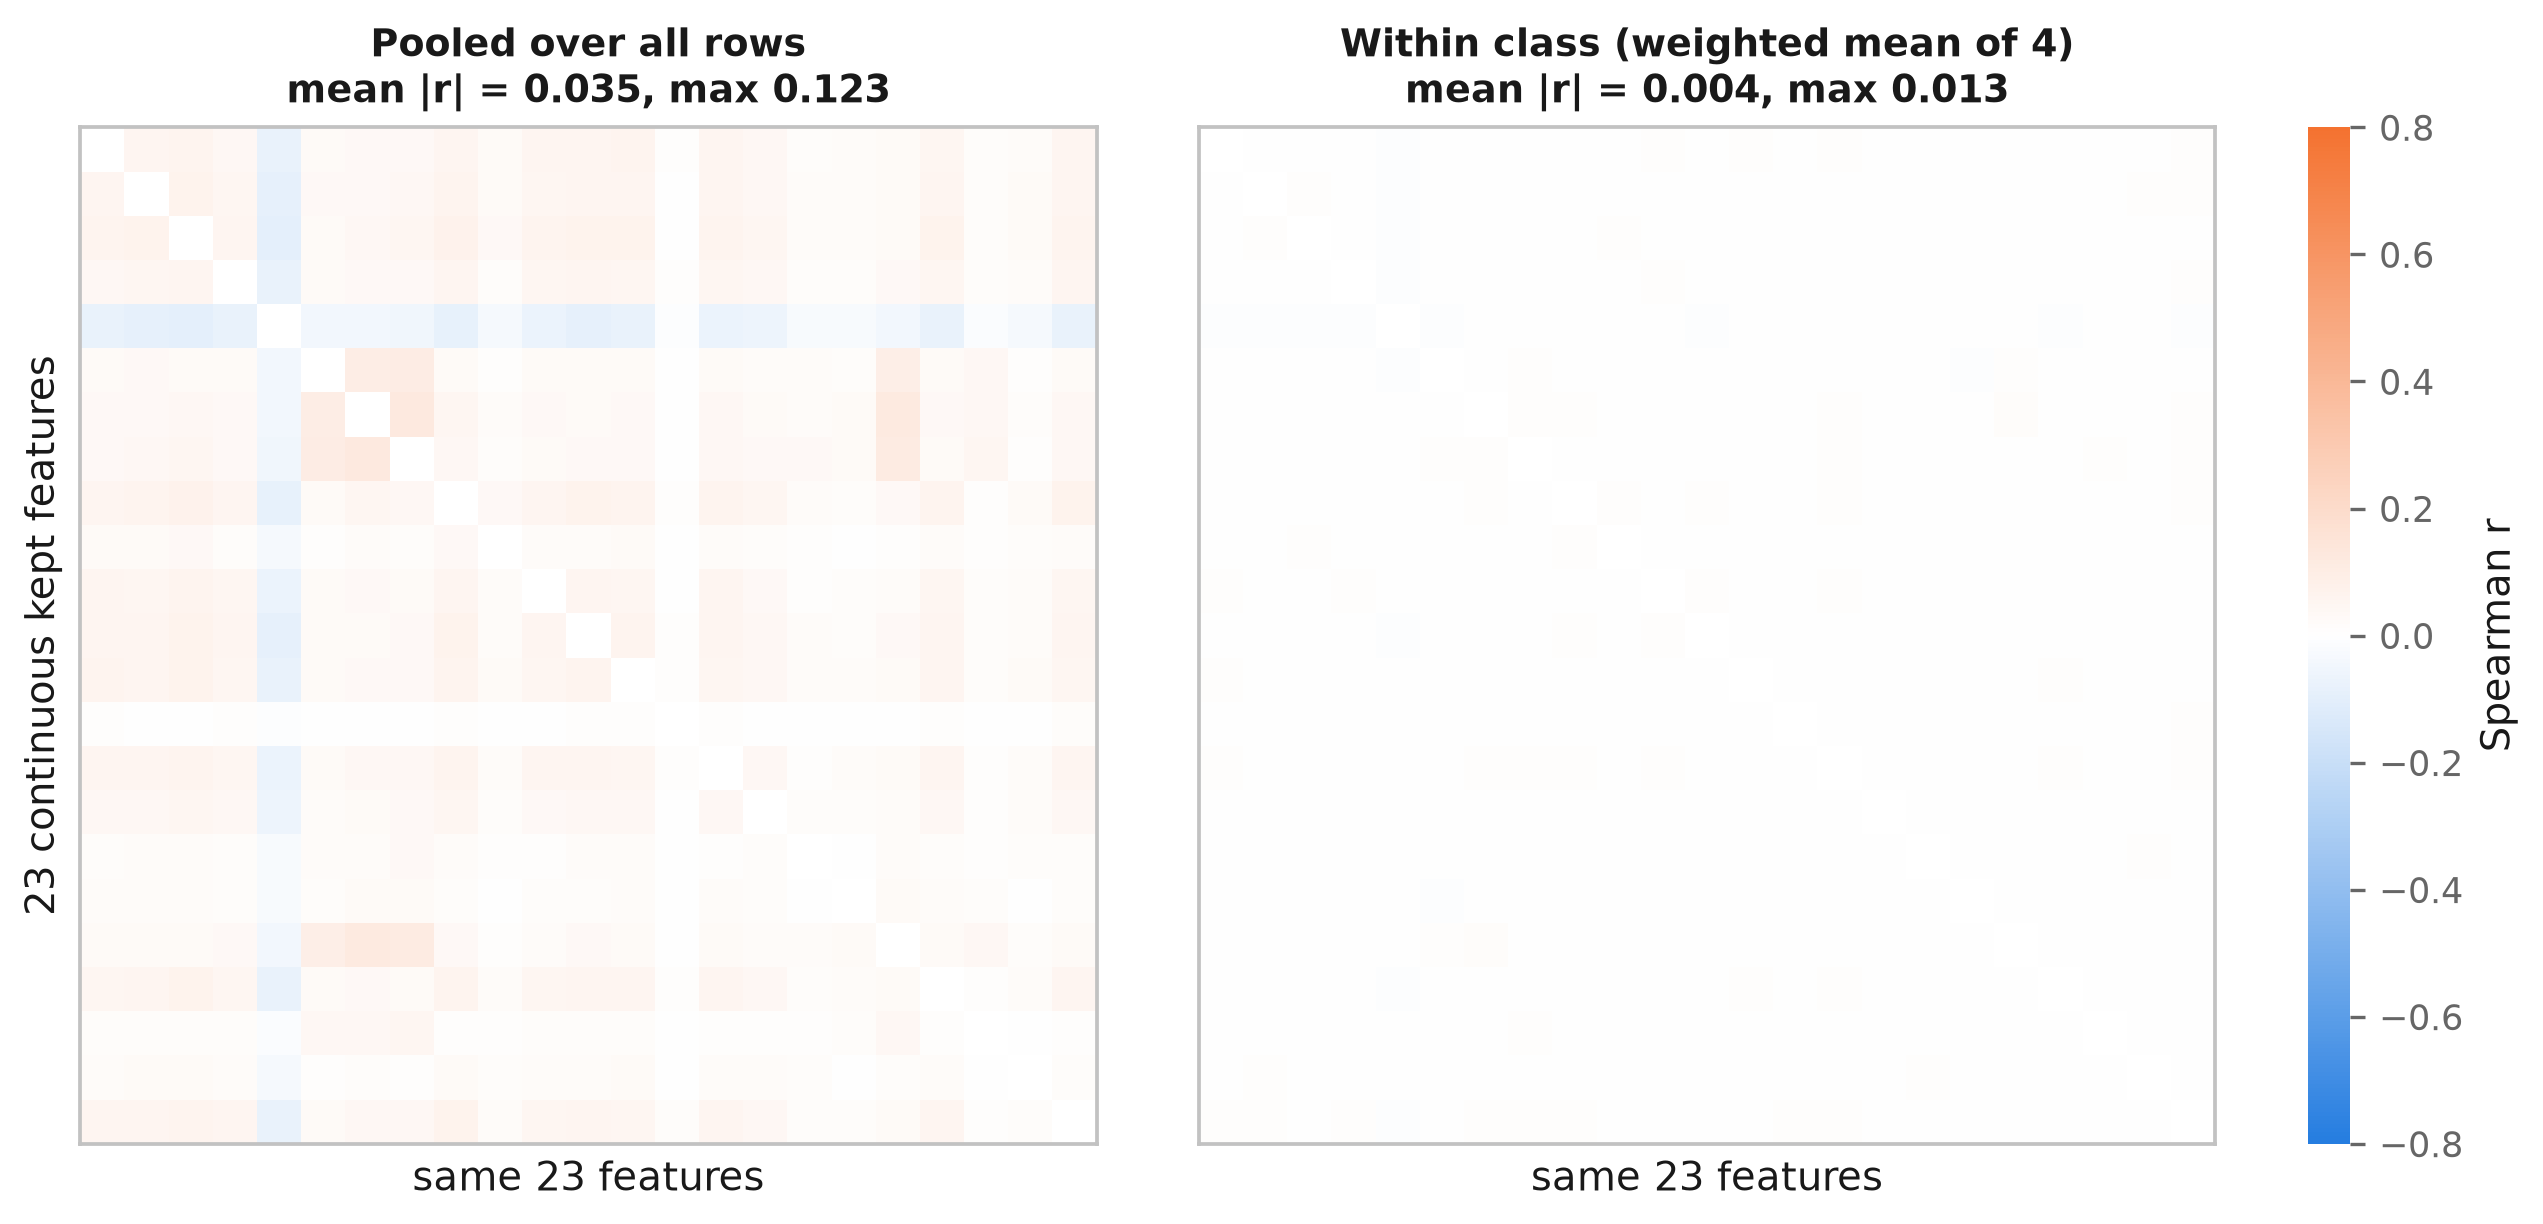
\includegraphics[width=\linewidth,height=0.33\textheight,keepaspectratio]{fig_t2_independence.png}
\caption{Spearman correlation among the 23 continuous kept features (diagonal masked). Left: all rows pooled. Right: weighted mean of the four within-class matrices. Conditioning on the class removes almost all correlation.}
\label{fig:t2-indep}
\end{figure}

\emph{What we see.} Pooled over all rows the mean absolute correlation is 0.035 (maximum 0.123). Inside a class it falls to 0.0036 (maximum 0.013), a 9.6-fold drop. The median absolute Pearson correlation per class is 0.004--0.010. The features are therefore conditionally independent given the segment, up to noise. Under that structure Naive Bayes \citep{naivebayes} is the Bayes-optimal classifier, because the joint likelihood is exactly the product of the one-dimensional likelihoods. \emph{What we decided.} Use a histogram Naive Bayes model as the main component, with a nonparametric density per feature, instead of a high-capacity model that would have to learn independence from data.

\paragraph{The latent 2$\times$2 grid.} Figure~\ref{fig:t2-latent} places the class medians of playtime and spending side by side, and relates the two informative categorical columns to the segment.

\begin{figure}[H]
\centering
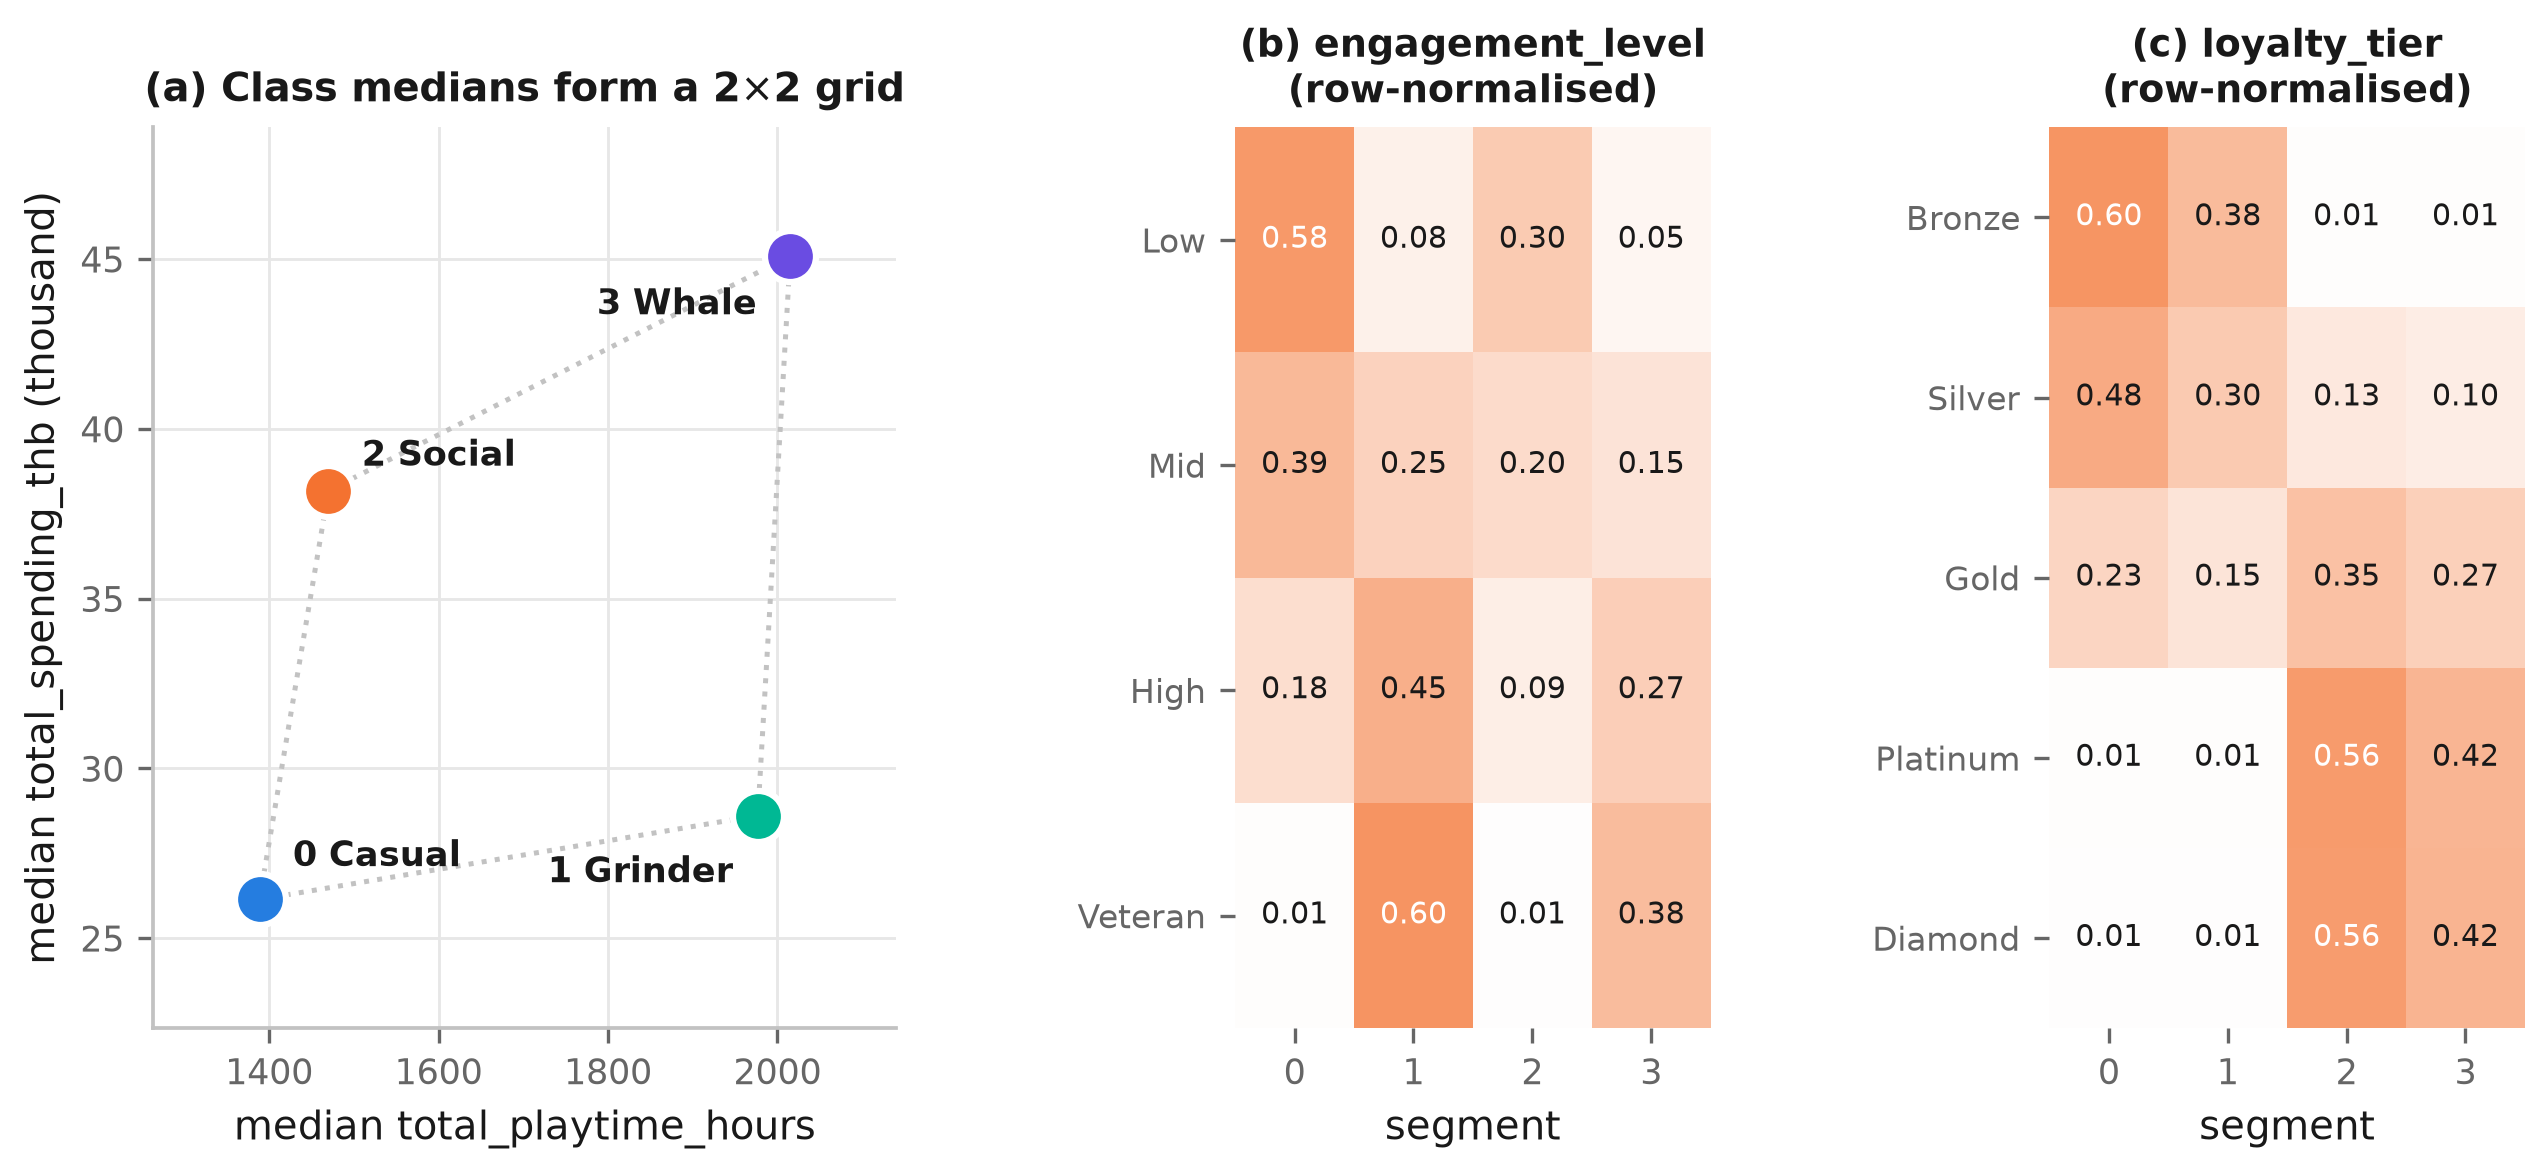
\includegraphics[width=\linewidth,height=0.33\textheight,keepaspectratio]{fig_t2_latent_2x2.png}
\caption{(a) Median lifetime playtime and spending of each segment. (b,c) Distribution of the segment within each level of \texttt{engagement\_level} and \texttt{loyalty\_tier} (rows sum to 1).}
\label{fig:t2-latent}
\end{figure}

\emph{What we see.} The four medians sit at the corners of a rough grid: Casual and Social play fewer hours (1{,}389 h and 1{,}470 h), Grinder and Whale more (1{,}977 h and 2{,}015 h); Casual and Grinder spend less (26.1k and 28.6k THB), Social and Whale more (38.2k and 45.1k THB). The segment is therefore two binary traits, engagement and spending, and the two categorical columns are noisy read-outs of them: a \texttt{Veteran} is almost never Casual or Social (1\% each), and \texttt{Platinum} and \texttt{Diamond} players are almost never Casual or Grinder (1\% each). Yet no level is perfectly pure: those small residual cells hold the players whose label disagrees with their profile. \emph{What we decided.} We treat these rows as label noise \citep{noisylabels} and model it explicitly with an EM step (Section~\ref{sec:t2-design}). Two observations support the reading that they are random label flips rather than a real fifth type of player. First, a row that is inconsistent inside its class (a Casual player with engagement \texttt{Veteran} or loyalty \texttt{Diamond}) carries the \emph{feature profile} of the other class, 0.4 to 1.2 standard deviations away from its labelled class. Second, the within-class feature correlations stay below 0.013, so these rows are not a hidden sub-population with its own dependence structure. We let the EM step estimate the flip rate (2.8\%, which is the value we quote for the estimate; Section~\ref{sec:t2-design} reconciles it with the roughly 3\% that the first release revealed) rather than fixing it. We also tested merging the densities along the two axes; the data rejected it for most features (Section~\ref{sec:t2-mistakes}).

\subsubsection{Data Preprocessing}

Preprocessing is deliberately small. The EDA findings translate into the decisions in Table~\ref{tab:t2-evidence}.

\begin{evidencetable}{EDA evidence and the pipeline decision it motivated (task 2).}{tab:t2-evidence}
Figure~\ref{fig:t2-balance}a. Classes are 39/25/20/15\% and the metric weighs them equally & Fit an affine macro-F1 decision rule on out-of-fold probabilities instead of using \texttt{argmax}. \\
Figure~\ref{fig:t2-balance}b. About 7.7\% missing in every feature and class & Skip a missing value in the likelihood (marginalise it); no imputation in the Naive Bayes model. \\
Figure~\ref{fig:t2-signal}. 16 columns have no relation to the segment & Drop \feat{player_id} and the 16 noise columns; keep 28 features. \\
Figure~\ref{fig:t2-indep}. Within-class correlation is $\approx$0 & Histogram Naive Bayes with per-feature densities is the main model (weight 0.87). \\
Figure~\ref{fig:t2-latent}. Two latent traits, noisy categorical read-outs, a few contradictory cells & Explicit label-noise EM inside Naive Bayes; add a spline logistic regression and an MLP for residual structure. \\
\end{evidencetable}

\paragraph{Feature set.} Of the 44 raw features we keep 28: 23 continuous ones and five discrete ones (\feat{competitive_rank}, \feat{watches_esports}, \feat{vip_tier}, \feat{engagement_level}, \feat{loyalty_tier}). The dropped columns are \feat{random_metric_1..3}, \feat{account_age_days}, \feat{responds_to_discounts}, \feat{item_type_preference_social}, \feat{avg_match_length}, \feat{preferred_game_mode}, \feat{region}, \feat{platform}, \feat{device_type}, \feat{payment_method}, \feat{language}, \feat{account_status}, \feat{player_type_tag} and \feat{skill_tier}.

\paragraph{Naive Bayes inputs.} Bin edges are the quantiles of the training portion of each fold only, so no information flows from the validation rows. Discrete features use empirical categorical PMFs with Laplace smoothing $\alpha=1$ (with an explicit \texttt{NA} level for the two string columns), avoiding arbitrary ordinality assumptions. A missing continuous value contributes a log-likelihood of zero. This is safe because the missingness is completely at random \citep{mcar}: the NaN rate is 7.5--8\% in every feature and every class, and the number of NaNs per row is equal across classes. There is no scaling and no imputation.

\paragraph{Inputs of the two discriminative models.} In contrast to Naive Bayes, the spline logistic regression and the MLP require dense numerical representations. They use the numeric columns that survive the screen, plus one-hot encoding for the categorical features \feat{engagement_level} and \feat{loyalty_tier}. Inside every training fold, missing values are filled with the fold median, then a quantile transformer maps each feature to a normal distribution and a scaler standardises it. Every transformer is fitted on the training part of its fold.

\subsubsection{Model Design}
\label{sec:t2-design}

The final model is a three-part probabilistic blend followed by a decision rule tuned for macro F1 (Figure~\ref{fig:t2-pipeline}, Table~\ref{tab:t2-models}).

\begin{figure}[H]
\centering
\begin{tikzpicture}[x=1cm,y=1cm]
\node[stage] (raw) at (0,0) {Raw data\\104{,}000 rows, 44 features};
\node[stage,fill=\taskcolor{2}!14] (drop) at (5.4,0) {Drop \feat{player_id} and 16 noise columns\\28 features};
\node[stage] (cv) at (10.8,0) {Stratified 5-fold split\\seed 42, training rows only inside each fit};
\node[model,draw=\taskcolor{2},thick] (nb) at (0,-3.4) {\textbf{EM histogram Naive Bayes} (0.87)\\bins and smoothing per feature by inner 4-fold log-loss; NaN skipped; 15 EM steps for label noise};
\node[model] (lr) at (5.4,-3.4) {\textbf{Spline logistic regression} (0.08)\\6-knot cubic splines, $C=0.05$};
\node[model] (mlp) at (10.8,-3.4) {\textbf{MLP} (0.05)\\128-64 SiLU, dropout 0.2, 12 epochs};
\node[stage,text width=12cm] (blend) at (5.4,-5.8) {Probability blend $0.87\,p_{\mathrm{NB}}+0.08\,p_{\mathrm{LR}}+0.05\,p_{\mathrm{MLP}}$};
\node[stage] (fit) at (0,-8.0) {Fit $(a_k,b_k)$ by fixed point on out-of-fold probabilities};
\node[decision,draw=\taskcolor{2},thick] (aff) at (5.4,-8.0) {Affine macro-F1 rule\\$\arg\max_k\; a_k p_k+b_k$};
\node[stage,fill=\taskcolor{2}!14] (out) at (10.8,-8.0) {Segment 0--3 for each test player};
\draw[flow] (raw) -- (drop);
\draw[flow] (drop) -- (cv);
\coordinate (bus) at (10.8,-1.7);
\draw[thick,ink!75] (cv.south) -- (bus);
\draw[thick,ink!75] (bus) -- (0,-1.7);
\draw[flow] (0,-1.7) -- (nb.north);
\draw[flow] (5.4,-1.7) -- (lr.north);
\draw[flow] (bus) -- (mlp.north);
\draw[flow] (nb.south) -- (nb.south |- blend.north);
\draw[flow] (lr.south) -- (lr.south |- blend.north);
\draw[flow] (mlp.south) -- (mlp.south |- blend.north);
\draw[flow] (blend.south) -- (aff.north);
\draw[flow] (fit) -- (aff);
\draw[flow] (aff) -- (out);
\node[note,anchor=north] at (5.4,-9.0) {$a_k=2/(\pi_k+q_k)$ and $b_k=-F_k/(\pi_k+q_k)$ use out-of-fold predictions only; the same values are applied to the test set};
\end{tikzpicture}
\caption{Task 2 pipeline from raw features to predicted segments.}
\label{fig:t2-pipeline}
\end{figure}

\begin{table}[H]\centering\small
\caption{Components of the final Task 2 model.}\label{tab:t2-models}
\begin{tabular}{@{}L{.20\linewidth}L{.09\linewidth}L{.62\linewidth}@{}}
\toprule
\textbf{Component} & \textbf{Weight} & \textbf{Training and settings} \\
\midrule
EM histogram Naive Bayes & 0.87 & Per continuous feature, bins from training quantiles and Gaussian smoothing. The bin count (64, 128 or 256) and the smoothing width ($\sigma\in\{3,4,6,8,12\}$) are chosen per feature by an inner 4-fold search on the log-loss of the one-feature posterior. Laplace $\alpha=1$. Missing values skipped. \\
Spline logistic regression & 0.08 & Cubic spline basis with 6 quantile knots on the numeric inputs plus one-hot categoricals; $C=0.05$, 300 iterations. \\
MLP & 0.05 & Two hidden layers (128, 64) with SiLU and dropout 0.2, AdamW, one-cycle schedule, 12 epochs, batch 512. \\
Decision rule & --- & Affine score $a_kp_k+b_k$ per class; $(a_k,b_k)$ solved by 8 fixed-point iterations on the OOF probabilities. \\
\bottomrule
\end{tabular}
\end{table}

\paragraph{EM histogram Naive Bayes.} The class posterior is $P(z\mid x)\propto \pi_z\prod_j p_j(x_j\mid z)$, taken over the observed features only. The one-dimensional densities are histograms, so the model assumes no parametric shape. Choosing the bin count and the smoothing by the log-loss of the one-feature posterior judges calibration directly, so the choice does not depend on bin width. Tuning the smoothing of every feature against the F1 of the classifier overfitted the folds, and we replaced that earlier approach (Section~\ref{sec:t2-mistakes}).

To handle label noise, we assume that the observed label $\tilde y$ equals the latent segment with probability $1-\varepsilon$ and otherwise takes one of the other three at random. Fifteen EM steps alternate between computing each row's posterior over the latent class from its features, the prior and the noise model (E-step), and re-estimating the histograms from those soft assignments (M-step); the noise rate $\varepsilon$ is updated from the same posteriors. The fitted flip rate is stable across folds (0.0280--0.0288, and 0.0284 on the full new-release data). At prediction time the latent posterior is mapped through the noise matrix to a probability for the observed label.

\emph{Estimated versus true flip rate.} Throughout this report 2.8\% is the rate that EM estimates from the labels and the features alone, and about 3\% is the true rate of the generator. The true rate was measured once, on the first release, where the leaked \feat{player_id} blocks gave the class of every row: 3.0\% of the training labels disagreed with their block, spread uniformly over the other three classes ($\chi^2$ $p$ between 0.44 and 0.84). The EM estimate on that release was 0.028 (E06 of our experiment log), so it falls 0.2 points short of the truth, which is plausible because EM can only recognise a flip when the features disagree with the label. A label-noise model matters for \emph{calibration}, not for the decision: Naive Bayes trained on the id-cleaned labels reaches 0.7560 against 0.7557 on seed 42, and the argmax decisions do not change, whereas the EM-NB lowers the log-loss from 0.6229 to 0.5993 with density selection held equal (first release). The EM step is therefore kept for its probabilities, which the blend and the affine rule consume, and it adds about $+0.0004$ of macro F1 on top.

\paragraph{Spline LR and MLP.} The spline logistic regression uses a cubic spline basis \citep{splines} and is fitted with scikit-learn \citep{sklearn}; the MLP is trained in PyTorch \citep{pytorch}. These two models cost little and capture smooth structure that Naive Bayes ignores. Their weights (0.08 and 0.05) come from earlier nested blend work on the first data release; re-tuning them on the new data with nested cross-validation gave $+0.00006\pm0.00018$, so we kept the original weights.

\paragraph{Affine macro-F1 rule.} The class-$k$ F1 can be written $F_k=2\,P(y=k,\hat y=k)/(\pi_k+q_k)$ with $\pi_k$ the true share and $q_k$ the predicted share. Differentiating macro F1 around an operating point shows that predicting class $k$ for a row adds, to first order, $\bigl(2p_k-F_k\bigr)/(\pi_k+q_k)$ to the total. Predicting $\arg\max_k a_kp_k+b_k$ with $a_k=2/(\pi_k+q_k)$ and $b_k=-F_k/(\pi_k+q_k)$ therefore maximises macro F1 near that point, where $q_k$ and $F_k$ are themselves produced by the rule. We start from $q=\pi$ and $F_k=0.75$ and iterate eight times on the OOF probabilities. The converged coefficients are about $a=(2.50, 3.98, 5.00, 6.74)$ and $b=(-1.02,-1.49,-1.79,-2.52)$: the rule pushes the rare classes up. We then apply the same fixed $(a_k,b_k)$ to the test probabilities, so no test statistic enters.

\paragraph{Validation.} Five stratified folds with seed 42. Density selection, transformer fitting and EM are repeated inside each fold, and the blend weights and the affine rule are fixed from the OOF predictions. The test probabilities come from a refit on the full training set for Naive Bayes and from the average of the five fold models for the other two.

\subsubsection{Evaluation and Results}
\label{sec:t2-eval}

The score is $\text{macro F1}=\frac14\sum_{k=0}^{3}\frac{2\,\text{TP}_k}{2\,\text{TP}_k+\text{FP}_k+\text{FN}_k}$. Table~\ref{tab:t2-results} lists the out-of-fold macro F1 of each component and of the final prediction. The tuned LightGBM baseline (0.7524) was measured on the first data release, so it appears in Table~\ref{tab:t2-failed} instead and is not compared with these numbers.

\begin{table}[H]\centering\small
\caption{Out-of-fold macro F1 on the re-released Task 2 data (5 folds, seed 42, no \texttt{player\_id}).}\label{tab:t2-results}
\begin{tabular}{@{}L{.50\linewidth}L{.17\linewidth}L{.22\linewidth}@{}}
\toprule
\textbf{Model (new data)} & \textbf{OOF macro F1} & \textbf{Difference to EM-NB alone} \\
\midrule
MLP (weight 0.05) & 0.75227 & $-0.00539$ \\
Spline logistic regression (0.08) & 0.75468 & $-0.00298$ \\
EM histogram Naive Bayes (0.87) & 0.75766 & reference \\
Blend 0.87 / 0.08 / 0.05, \texttt{argmax} & 0.75798 & $+0.00032$ \\
\textbf{Blend + affine rule (final)} & \textbf{0.75826} & $+0.00060$ \\
\bottomrule
\end{tabular}
\end{table}

The Naive Bayes model alone reaches 0.75766 (per fold 0.7548--0.7617; three seeds 0.7577--0.7582). The two discriminative models are individually worse by 0.003--0.005 but make different mistakes, so the 0.87/0.08/0.05 blend adds 0.00032 over Naive Bayes alone, and the affine rule, which changes 2{,}056 of the 104{,}000 OOF predictions (1.98\%), adds a further 0.00028. The final pipeline reaches an OOF macro F1 of 0.75826. All numbers in this table come from the re-released data; the experiments of the failed-experiments table and the decision log are labelled ``first release'' or ``new data'' row by row, and the two releases must not be compared absolutely, because the rows were regenerated. The public leaderboard agrees in direction. On the first data release, replacing the plain Naive Bayes in Task~2 by the blend and the rule raised the public score from 0.71965 to 0.71999 (\texttt{sub\_v16b} $\to$ \texttt{sub\_v18a}), a gain of 0.00034 on the whole submission, or about 0.0017 of Task~2 macro F1 at a task weight of 0.2. The submission that this report describes, with the same Task~2 model, scored 0.87351 on the public leaderboard.

\paragraph{Decision log.} Figure~\ref{fig:t2-decision-log} lists every Task~2 experiment, with the metric each number measures. The rows are in \texttt{data/decision\_log\_t2.csv}.

\begin{figure}[p]
\centering
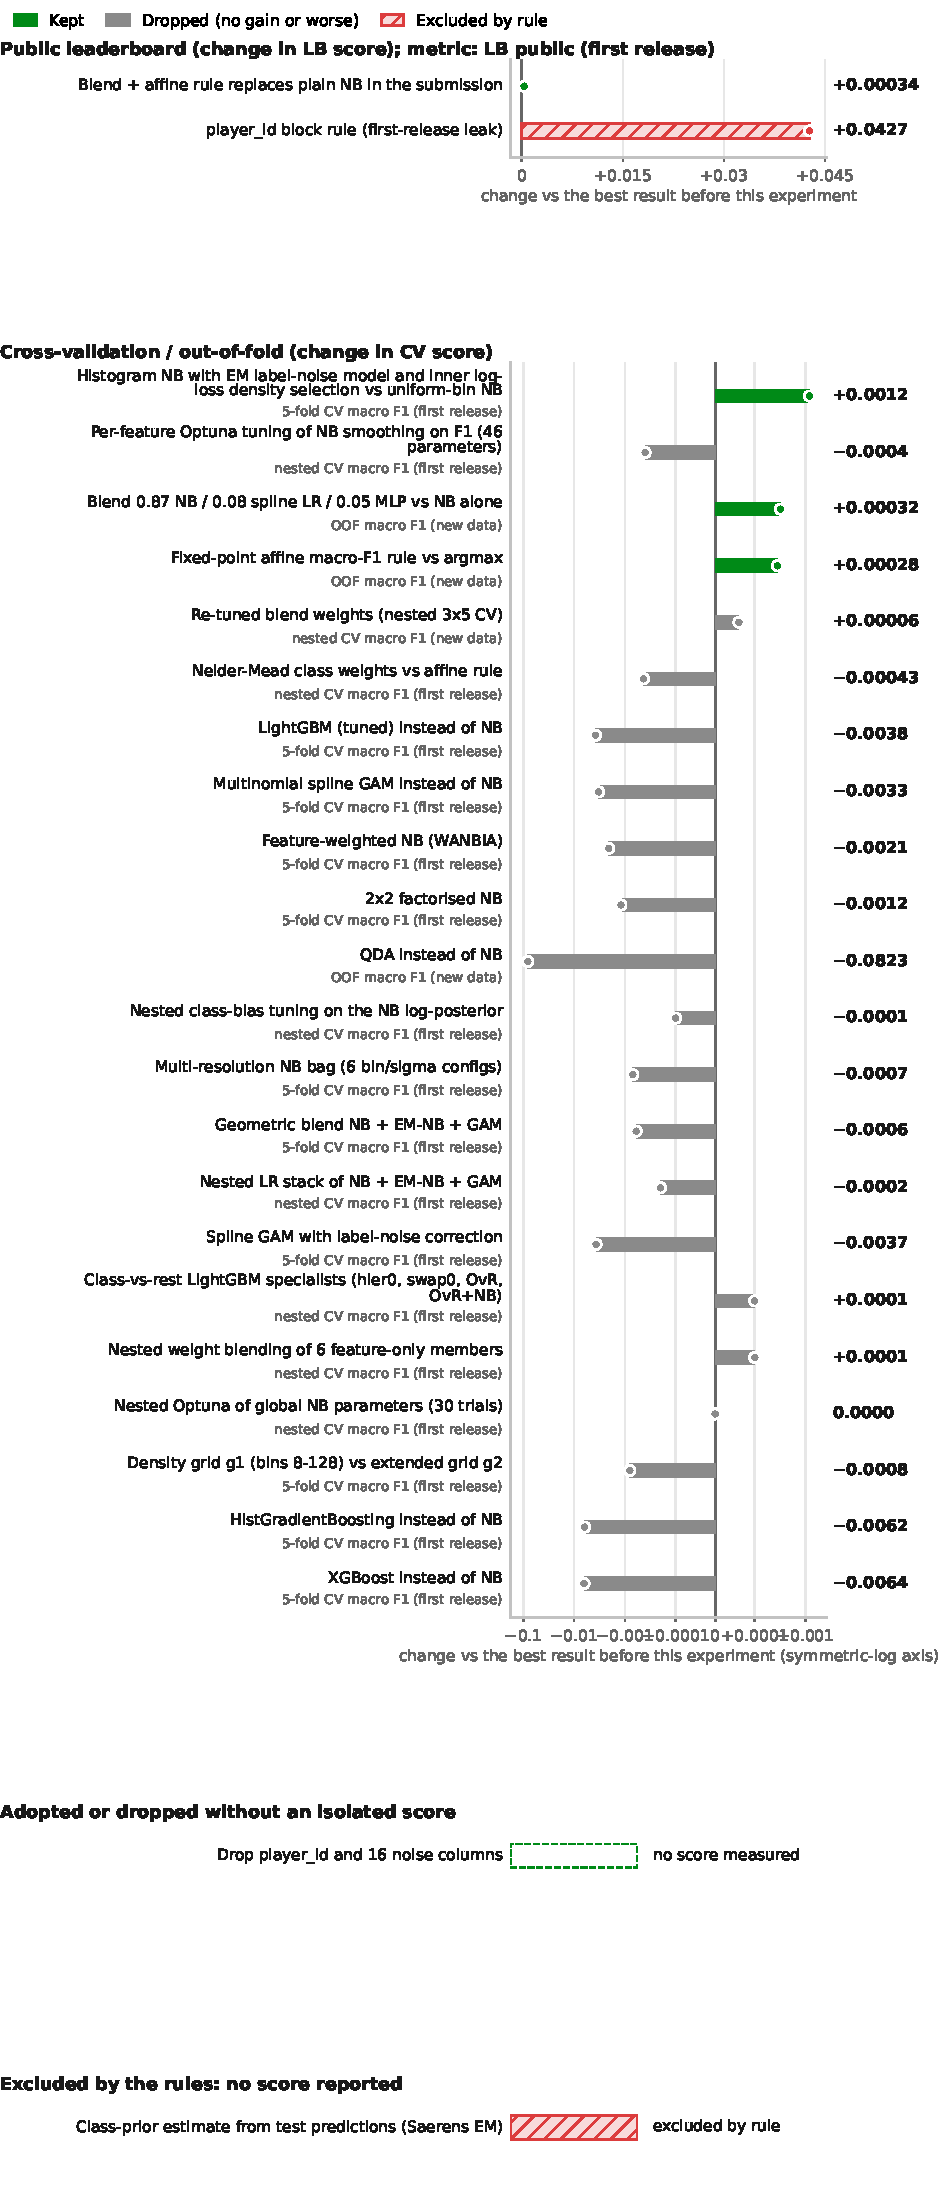
\includegraphics[width=\linewidth,height=0.85\textheight,keepaspectratio]{decision_log_t2.pdf}
\caption{Task 2 decision log: change in score (one panel per metric family) per experiment, kept versus dropped versus rule-excluded. Green = kept, grey = dropped, red hatched = excluded by the competition rules.}
\label{fig:t2-decision-log}
\end{figure}

\subsubsection{Insights from Model Behaviour}

Figure~\ref{fig:t2-errors} opens up the final OOF predictions.

\begin{figure}[H]
\centering
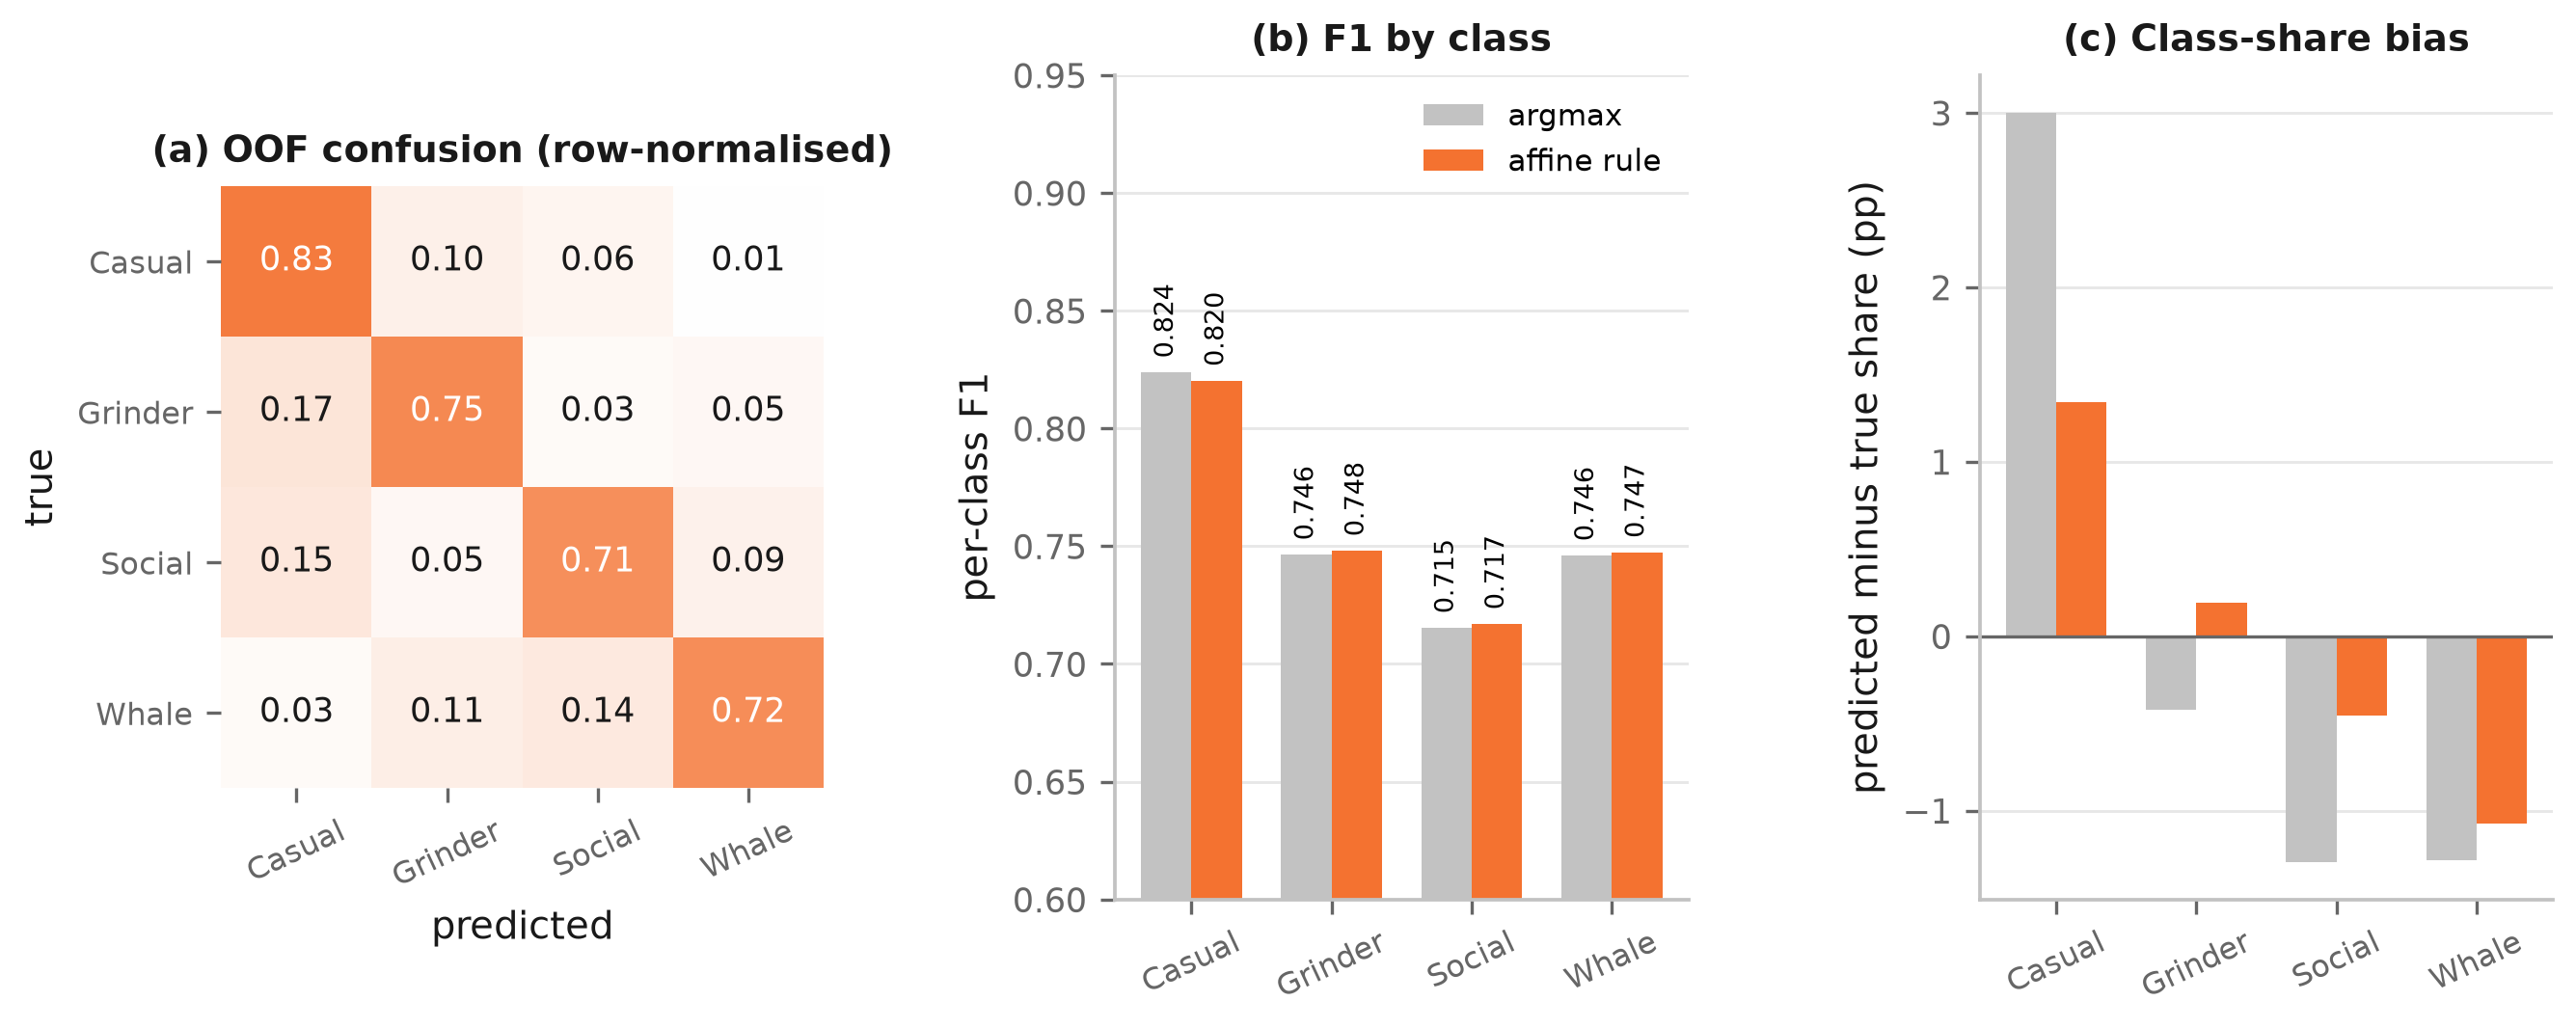
\includegraphics[width=\linewidth,height=0.33\textheight,keepaspectratio]{fig_t2_errors.png}
\caption{(a) Row-normalised confusion matrix of the final OOF predictions. (b) Per-class F1 with plain \texttt{argmax} on the blend versus the affine rule. (c) Predicted minus true class share. The rule shrinks the over-prediction of the Casual class from +3.0 to +1.3 points.}
\label{fig:t2-errors}
\end{figure}

\paragraph{Where the model errs.} The F1 scores are 0.820 (Casual), 0.748 (Grinder), 0.717 (Social) and 0.747 (Whale). The confusions follow the latent grid of Figure~\ref{fig:t2-latent}: 17\% of Grinders are called Casual and 14\% of Whales are called Social, which are neighbours that share one trait. The opposite corners (Casual with Whale, Grinder with Social) are confused by 5\% or less. Social is the hardest class, with a recall of 0.709: 15\% of its players look Casual and 9\% look Whale.

\paragraph{What the rule does.} With \texttt{argmax}, the Casual class is over-predicted by 3.0 points and the three others are under-predicted. The affine rule re-balances the shares to $+1.3$, $+0.2$, $-0.5$ and $-1.1$ points and trades 0.0035 of Casual F1 for gains in the other three classes. That is the purpose of a macro metric. The test predictions have the same shape (40.9, 25.4, 19.4 and 14.4\% against 39.4, 25.0, 20.2 and 15.4\% in training), which indicates that the test mix is close to the training mix and the rule is not tuned to a shifted prior.

\paragraph{Confidence.} The Naive Bayes probabilities are well calibrated (OOF log-loss 0.5975 on the new data). The 31\% of players whose blended top probability is at least 0.9 are classified correctly 94.8\% of the time, against 77.1\% overall. This ordering is useful in practice: a campaign can restrict itself to confident predictions.

\paragraph{Ceiling.} Tuning, richer models and extra components all landed within 0.001 of the Naive Bayes score. We read this as a data ceiling. The generator gives conditionally independent features and a flip rate of about 3\% (2.8\% as estimated by EM); even a perfect model of the latent class would mislabel that fraction of the rows, and the overlapping tails cost the rest. A learning curve supports the reading. Figure~\ref{fig:t2-lc} trains the histogram Naive Bayes on a growing share of each fold's training part (first-release data, three seeds). Macro F1 rises from 0.7460 at 8{,}320 rows to 0.7518 at 20{,}800, 0.7539 at 41{,}600, 0.7550 at 62{,}400 and 0.7557 at 83{,}200 rows, so each doubling of the data brings less (about $+0.0018$ for the last one), and the extrapolation to unlimited data leaves about 0.002 of headroom. The EM variant leads at small sizes (0.7472 against 0.7460 at 10\%) and the two merge at full size. Within the noise of one data set (about $\pm0.002$ for macro F1 on this many rows) we are therefore at the feature-only ceiling.

\begin{figure}[H]
\centering
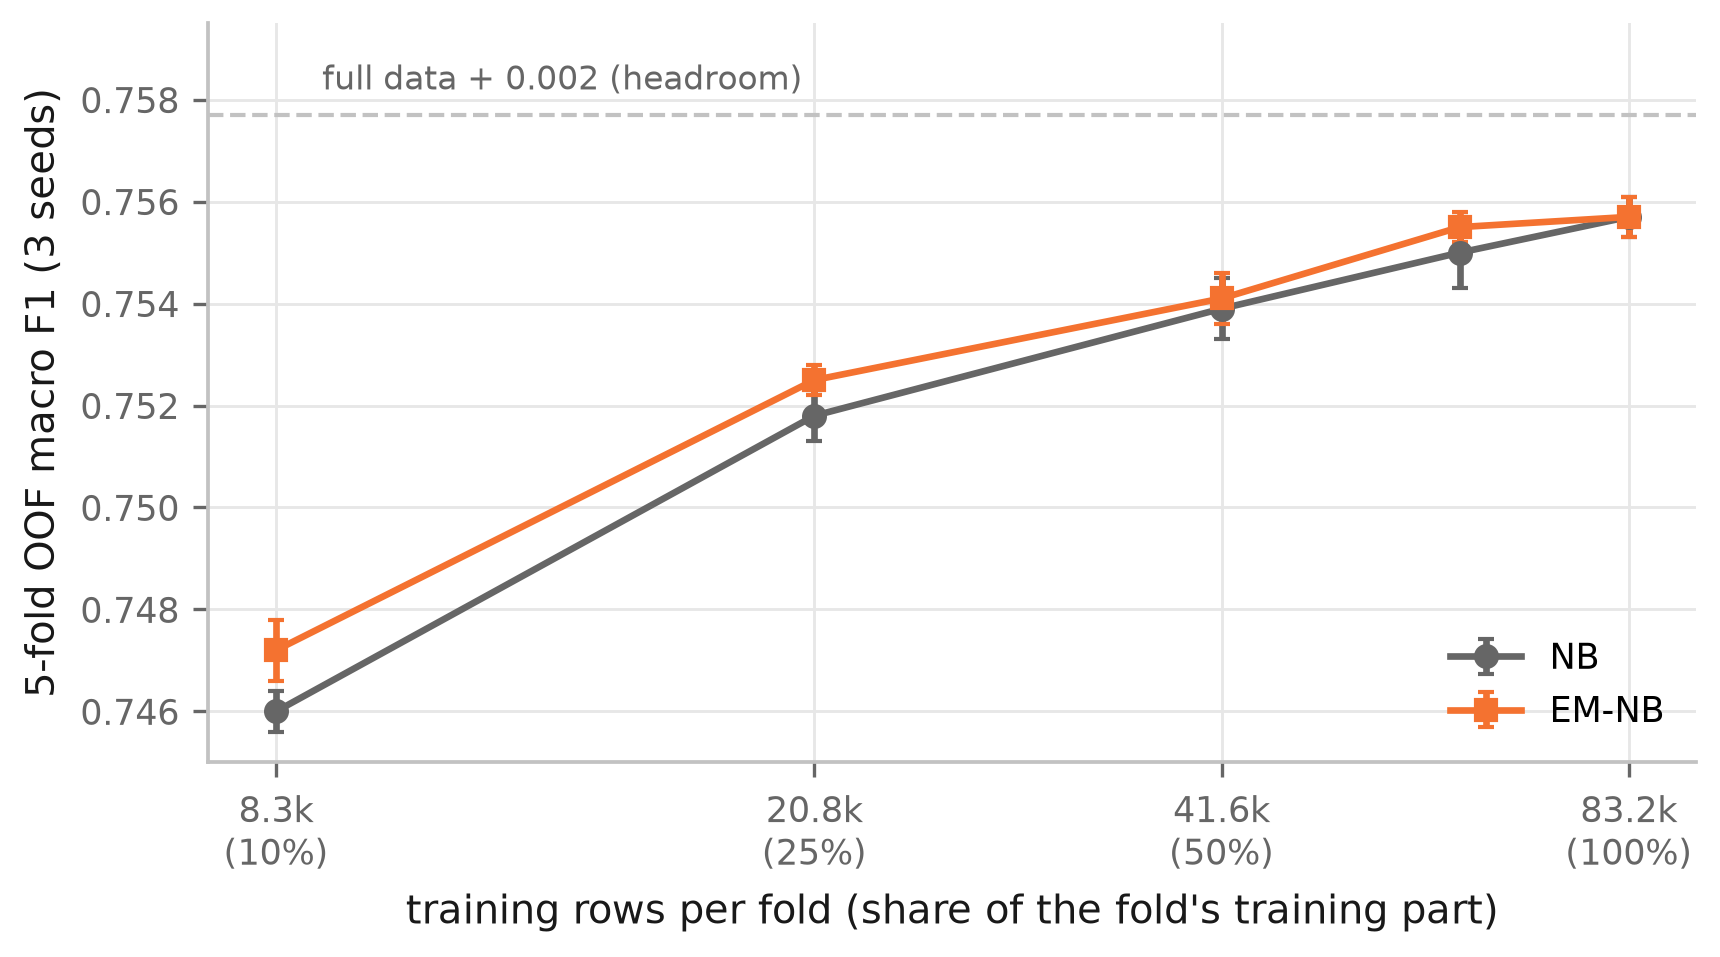
\includegraphics[width=.8\linewidth]{fig_t2_learning_curve.png}
\caption{Learning curve of the histogram Naive Bayes with and without the label-noise EM (first-release data; mean and standard deviation over 3 seeds). Hand-entered from the experiment log E11 in \texttt{data/t2\_learning\_curve.csv}.}
\label{fig:t2-lc}
\end{figure}

\subsubsection{Common Mistakes and Failed Experiments}
\label{sec:t2-mistakes}

\paragraph{The player-id leak (rule issue).} In the first data release the rows were ordered by class: \feat{player_id} fell into blocks of 40, 25, 20 and 15\% with exact cut points. A block rule on the id reached an out-of-fold macro F1 of 0.9677 against 0.756 for the honest model, and a public submission that used it scored 0.709, against 0.666 for the same file with the honest Naive Bayes in Task~2. The two files differed only in Task~2 and in the label format of Task~4, which the public leaderboard did not score at that time, so the gap of $+0.0427$ is the leak. We kept that file out of the clean pipeline and flagged the pattern to the teaching assistant. The organisers re-released the data on 12 November with the leak removed, and we confirmed that the id is now unrelated to the segment (one-vs-rest AUC 0.499--0.501). The honest pipeline kept improving on the new data (out-of-fold macro F1 0.75826 with the blend and the affine decision rule), so we dropped the leak and improved Task~2 only through the model and the decision rule. The teaching assistant later ruled that every prediction parameter must be computable without seeing the test set, so no id-based feature remains and no leak score appears in our headline tables. The lesson is to test every identifier and row order against the target before modelling, and to ask early when a pattern looks too good.

\paragraph{Tuning F1 directly.} We first tuned 46 smoothing parameters with Optuna \citep{optuna} against the macro F1 of the classifier. The nested estimate (0.7544) was below the untuned uniform histogram (0.7548 on the same seed), a sign of overfitting to the five folds. Selecting the density by the inner log-loss replaced it and gave 0.7558, then 0.7562 with the EM step (first-release data).

\paragraph{Models that lost to Naive Bayes.} Table~\ref{tab:t2-failed} lists the other experiments. Flexible discriminative models gained nothing from their capacity: LightGBM \citep{lightgbm} fit its training data to 0.7925 yet scored 0.7524 out of fold, and histogram gradient boosting and XGBoost \citep{xgboost} reached about 0.750 and 0.7498. Models that need more parameters than the generator provides (QDA) lost clearly. Specialist models, blends and extra tuning all tied with the final model within the noise bar of 0.001, so we kept the simplest member.

\begin{table}[H]\centering\small
\caption{Task 2 experiments that did not beat the final model. ``Data'' says which release the number was measured on: \emph{old} = first release, \emph{new} = 12 November re-release. Experiment codes E$n$ refer to our research log. Rows marked $^\dagger$ are scores of nested or multi-seed runs against the final 0.7562 (old).}\label{tab:t2-failed}
\begin{tabular}{@{}L{.30\linewidth}L{.07\linewidth}L{.17\linewidth}L{.36\linewidth}@{}}
\toprule
\textbf{Experiment} & \textbf{Data} & \textbf{Macro F1} & \textbf{Why it was dropped} \\
\midrule
LightGBM, tuned (E17b) & old & 0.7524 & Train score 0.7925: it overfits; there are no feature interactions to learn. \\
Histogram GB / XGBoost & old & 0.750 / 0.7498 & Same story as LightGBM. \\
Spline GAM \citep{splines} (E02) & old & 0.7529 & Better log-loss, worse F1 than Naive Bayes. \\
GAM with noise correction (E12) & old & 0.7525 & The correction fixes the log-loss (0.6029), not the F1. \\
Feature-weighted NB (WANBIA, E04) & old & 0.7539--0.7542 & Weighting a sum of equal log-likelihoods does not help. \\
2$\times$2 factorised NB (E09) & old & 0.7550 & The data rejected merging the densities along the two axes in 26 of 28 features. \\
Multi-resolution NB bag (E07) & old & 0.7555 & Averaging six bin and smoothing configurations adds nothing. \\
Class-vs-rest LightGBM specialists (E15) & old & 0.7537--0.7551$^\dagger$ & Their one-vs-rest AUC equals that of NB (0.931 / 0.923 / 0.924 / 0.940): nothing left to learn. \\
Class bias tuned on log-posterior (E01) & old & 0.7556$^\dagger$ & Tuned biases are about 0, so \texttt{argmax} is already F1-optimal. \\
Geometric blend / nested LR stack (E08) & old & 0.7556 / 0.7560$^\dagger$ & Gain of 0.0003 is below the noise bar. \\
Nested weight blending of 6 members (E16) & old & 0.7563$^\dagger$ & Tie; log-loss weights stable, F1-fitted weights unstable (sd 0.2). \\
Nested Optuna of global NB parameters (E17a) & old & 0.7562$^\dagger$ & Tie: the defaults already are the optimum. \\
Density grid at the edge (E14 g1) & old & 0.7554 & Picks sat on the grid boundary; extended grid g2 (kept) gained 0.0004. \\
LDA / QDA & new & 0.7337 / 0.6754 & Linear or full-covariance Gaussians do not fit the marginals. \\
Re-tuned blend weights, nested CV & new & $+0.00006$ & $\pm$0.00018, 8 of 15 folds improved: noise. \\
Nelder--Mead class weights & old & $+0.00019$ vs \texttt{argmax} & 0.00043 below the affine rule. \\
Class prior estimated from test predictions \citep{saerens} & old & no shift found & The estimated test prior equals the training prior; the TA ruling also bars this kind of step. \\
\bottomrule
\end{tabular}
\end{table}

\paragraph{The segment of Task 3.} The same player ids occur in Task~3, which also has a \feat{segment} column. We checked whether it could serve as extra labels: it agrees with the Task~2 segment of the same player at chance level (28\%), because the two files are independent draws from the generator. We did not use it.

\subsubsection{Domain Interpretation and Business Impact}

The situation in the brief is that Karena's marketing team runs generic campaigns that reach only 2--5\% of players and spends about 60 million baht a month. Casual players receive esports announcements and non-buyers receive item sales. A segment label lets each message go to the group that wants it. Table~\ref{tab:t2-playbook} turns the four segments into actions; the medians come from the training data and the shares from our test predictions.

\begin{table}[H]\centering\small
\caption{From segment to action. Medians are training medians; shares are predicted shares of the test players.}\label{tab:t2-playbook}
\begin{tabular}{@{}L{.12\linewidth}L{.10\linewidth}L{.17\linewidth}L{.50\linewidth}@{}}
\toprule
\textbf{Segment} & \textbf{Test share} & \textbf{Median hours / THB} & \textbf{Suggested use} \\
\midrule
0 Casual & 40.9\% & 1{,}389 / 26.1k & Low-friction campaigns: daily rewards, short modes; no esports promotion. \\
1 Grinder & 25.4\% & 1{,}977 / 28.6k & Ranked tournaments, esports events, skill items. \\
2 Social & 19.4\% & 1{,}470 / 38.2k & Friend-invite bundles, guild events, role-play invitations. \\
3 Whale & 14.4\% & 2{,}015 / 45.1k & VIP service, early access to rare items; no blanket discount codes. \\
\bottomrule
\end{tabular}
\end{table}

\paragraph{Cost of an error.} Not every mistake is equally harmful. The most common confusions are neighbours that share one trait (Grinder to Casual, Whale to Social), so a wrong campaign is usually partly relevant rather than irrelevant. The costly mistakes are Whales who are handled as Social players and miss VIP treatment (14\% of Whales) and the reverse, expensive concierge offers sent to players who will not respond. A practical design would send high-touch offers only to predictions with a top probability above a threshold, for example 0.9, which covers 31\% of players at 94.8\% accuracy, and use the general campaign for the rest. Macro F1 does not choose this threshold, because it weights all classes equally, whereas the real cost of missing a Whale is far larger than that of missing a Casual player. A production system should weight the errors by their revenue.

\paragraph{Deployment caveats.} The model relies on features that move with time (spending, login recency), and a segment is not a fixed trait, so predictions need a regular refresh, for example monthly. The label noise (estimated at 2.8\%, about 3\% in truth) means that even a perfect model will look wrong on a few percent of players; marketing tests should compare segment campaigns against a control group instead of reading single predictions as truth. Finally, the data is synthetic: the uplift of three to four times that the brief anticipates has to be measured on live players before it informs budgets.

\end{document}
